%% Common definitions, defined in sdss-er.tex
\newlength{\pointonesec}\settowidth{\pointonesec}{$0.1$ s}
\newlength{\acceptable}\settowidth{\acceptable}{Acceptable}

\newcommand{\sdssertable}{\begin{tabular}{|c|D{.}{.}{6.0}|D{.}{.}{6.0}|D{.}{.}{3.2}|}
\hline
\multicolumn{1}{|c|}{\textbf{Phase}} & \multicolumn{1}{c|}{\textbf{Images recognized}} & \multicolumn{1}{c|}{\textbf{Unrecognized}} &
\multicolumn{1}{c|}{\textbf{Percent recognized}} \\
\hline
\usnob: \makebox[\pointonesec][r]{$0.1$ s} & 172,882 & 9,339 & 94.87 \\
\usnob: \makebox[\pointonesec][r]{$1$ s} & 181,826 & 395 & 99.78 \\
\usnob: \makebox[\pointonesec][r]{$10$ s} & 182,158 & 63 & 99.97 \\
\usnob: \makebox[\pointonesec][r]{$15$ s} & 182,160 & 61 & 99.97 \\
\twomass & 182,211 & 10 & 99.99 \\
Original images & 182,221 & 0 & 100.00 \\
\hline
\end{tabular}
}

\newcommand{\sdsserradecfig}{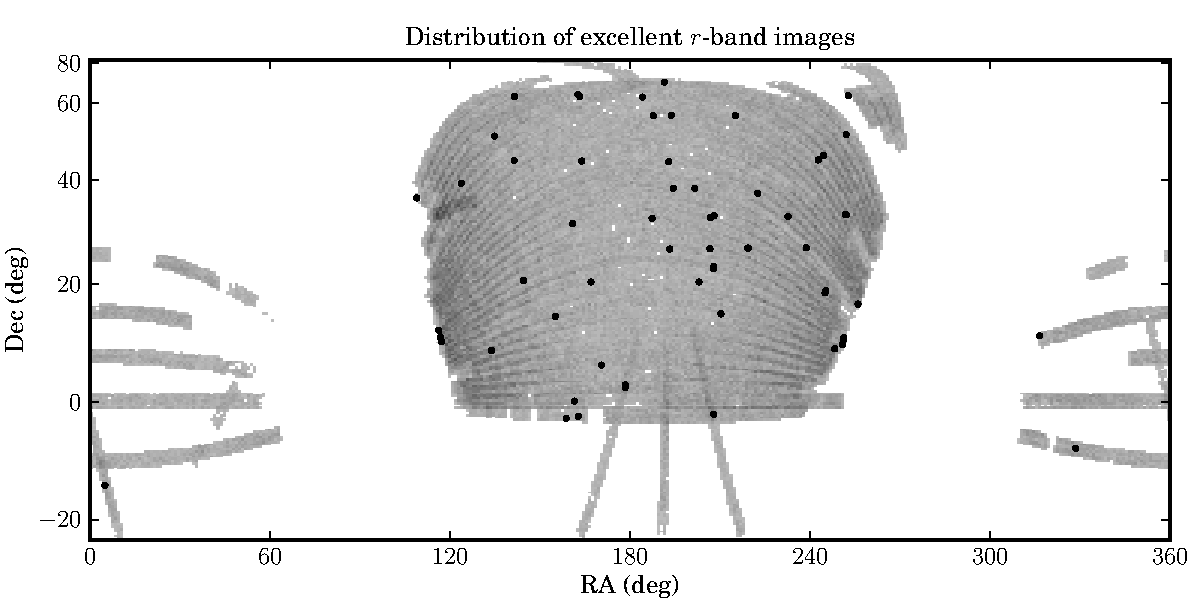
\includegraphics[width=2.000000\figunit]{sdss-er-radec}}
\newcommand{\sdssercputimefig}{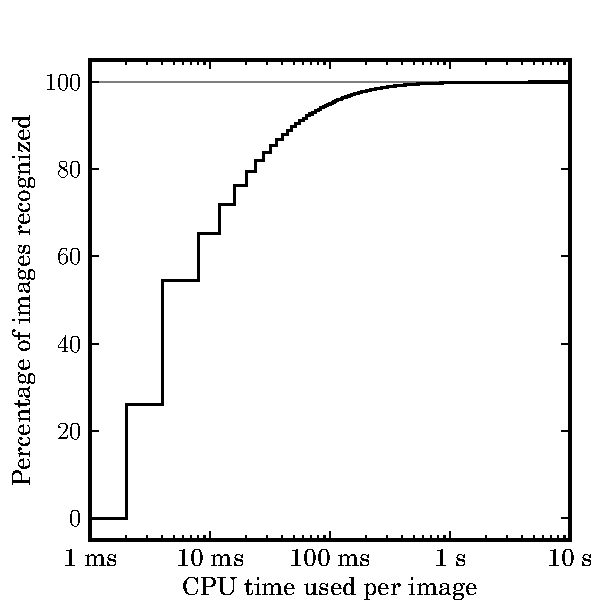
\includegraphics[width=1.000000\figunit]{sdss-er-cputime}}
\newcommand{\sdssernimagefig}{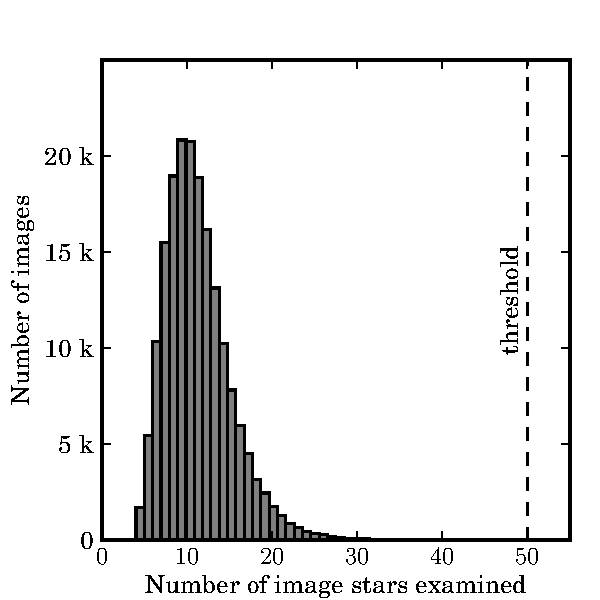
\includegraphics[width=1.000000\figunit]{sdss-er-nimage}}
\newcommand{\sdssernmatchfig}{\includegraphics[width=1.000000\figunit]{sdss-er-nmatch}}
\newcommand{\sdssercodeerrfig}{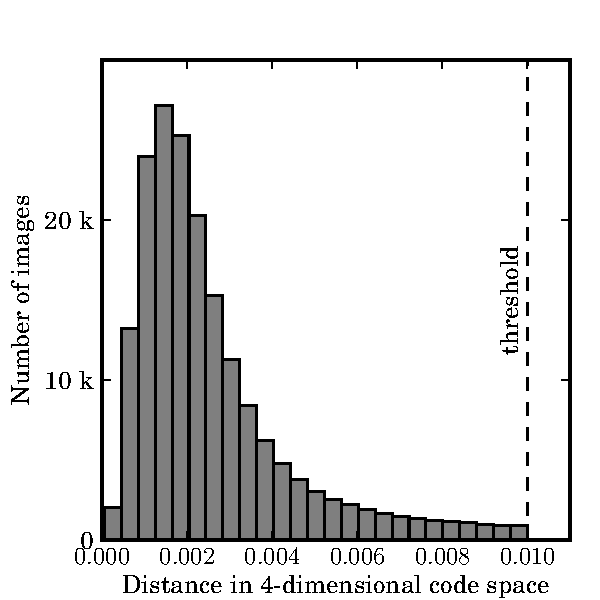
\includegraphics[width=1.000000\figunit]{sdss-er-codeerr}}
\newcommand{\sdsserbayesfig}{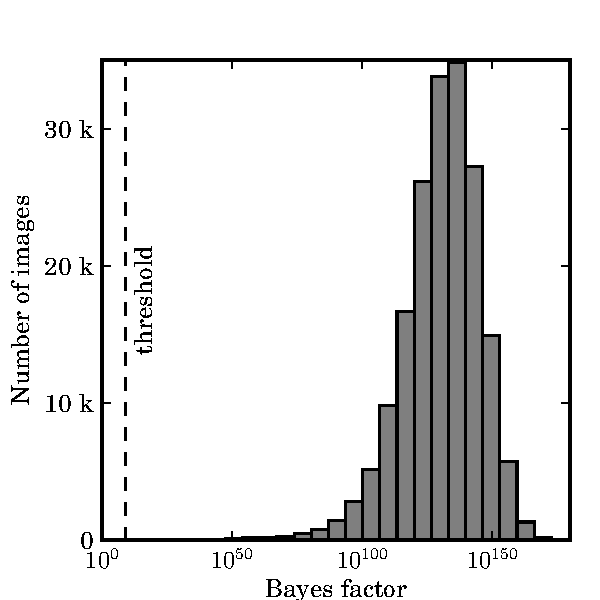
\includegraphics[width=1.000000\figunit]{sdss-er-bayes}}
